\documentclass[4paper]{article}
\usepackage[spanish]{babel}
%\usepackage[ansinew]{inputenc}
\usepackage[utf8x]{inputenc}
%\usepackage[utf-8]{inputenc}
%\usepackage[T1]{fontenc}
\usepackage{graphicx}
\usepackage{multicol}
\usepackage{float}
%\usepackage{longtable}
%\usepackage{array}
%\usepackage{multirow}
%\usepackage[latin1]{inputenc}
%\inputencoding{latin1}
\usepackage{hyperref}

\usepackage{color}

\definecolor{pblue}{rgb}{0.13,0.13,1}
\definecolor{pgreen}{rgb}{0,0.5,0}
\definecolor{pred}{rgb}{0.9,0,0}
\definecolor{pgrey}{rgb}{0.46,0.45,0.48}

\usepackage{listings}
\lstset{language=Java,
  showspaces=false,
  showtabs=false,
  breaklines=true,
  showstringspaces=false,
  breakatwhitespace=true,
  commentstyle=\color{pgreen},
  keywordstyle=\color{pblue},
  stringstyle=\color{pred},
  basicstyle=\ttfamily,
  moredelim=[il][\textcolor{pgrey}]{$$},
  moredelim=[is][\textcolor{pgrey}]{\%\%}{\%\%} 
}
\lstset{literate=
  {á}{{\'a}}1 {é}{{\'e}}1 {í}{{\'i}}1 {ó}{{\'o}}1 {ú}{{\'u}}1
  {Á}{{\'A}}1 {É}{{\'E}}1 {Í}{{\'I}}1 {Ó}{{\'O}}1 {Ú}{{\'U}}1
  {à}{{\`a}}1 {è}{{\`e}}1 {ì}{{\`i}}1 {ò}{{\`o}}1 {ù}{{\`u}}1
  {À}{{\`A}}1 {È}{{\'E}}1 {Ì}{{\`I}}1 {Ò}{{\`O}}1 {Ù}{{\`U}}1
  {ä}{{\"a}}1 {ë}{{\"e}}1 {ï}{{\"i}}1 {ö}{{\"o}}1 {ü}{{\"u}}1
  {Ä}{{\"A}}1 {Ë}{{\"E}}1 {Ï}{{\"I}}1 {Ö}{{\"O}}1 {Ü}{{\"U}}1
  {â}{{\^a}}1 {ê}{{\^e}}1 {î}{{\^i}}1 {ô}{{\^o}}1 {û}{{\^u}}1
  {Â}{{\^A}}1 {Ê}{{\^E}}1 {Î}{{\^I}}1 {Ô}{{\^O}}1 {Û}{{\^U}}1
  {œ}{{\oe}}1 {Œ}{{\OE}}1 {æ}{{\ae}}1 {Æ}{{\AE}}1 {ß}{{\ss}}1
  {ű}{{\H{u}}}1 {Ű}{{\H{U}}}1 {ő}{{\H{o}}}1 {Ő}{{\H{O}}}1
  {ç}{{\c c}}1 {Ç}{{\c C}}1 {ø}{{\o}}1 {å}{{\r a}}1 {Å}{{\r A}}1
  {€}{{\EUR}}1 {£}{{\pounds}}1
}
%$$

\renewcommand{\tablename}{Tabla}
\renewcommand{\S}{Conexión BD y Java }
\author{Manuel Molino Milla \and Luis Molina Garzón}
\title{\textbf{\S}}
\date{\today}

\begin{document}
\maketitle 
\tableofcontents
\newpage


\section{JDBC}
\subsection{Introducción}
\begin{itemize}
\item Es una API que nos permite conectar nuestra BD relacional con Java. 
\item Presenta un estándar para conectar a la BD.
\end{itemize}
\begin{figure}[H]
\centering
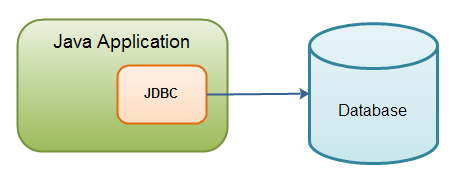
\includegraphics[scale=0.5]{imagenes/jdbc.png}
\end{figure}


\subsection{Componentes JDBC}
\begin{enumerate}
\item[JDBC Drivers] para cada SGBD tenemos nuestro propio \emph{driver} tenemos driver para \emph{mysql, sqlite, oracle, \dots}
\item[Connections] una vez conectado a la BD mediante el \emph{driver} podemos crear un objeto \emph{Connection} que establece la comunicación con la BD.
\item[Statements] objetos accesibles via objeto \emph{Connection} que nos permite consultas y actualizaciones de la BD.
\item[ResultSets] una vez realizada la consulta via \emph{Statements} obtenemos objetos de este tipo.
\end{enumerate}


\subsection{Cargando el driver, estableciendo la conexión y cerrándola}
Para las versiones de JDBC anteriores al 4. hay que cargar el driver, previamente hay que descargar el jar correspondiente
\begin{lstlisting}
Class.forName("com.mysql.jdbc.Driver"); //en el caso de mysql
Class.forName("org.h2.Driver"); //para h2Database
Class.forName("org.sqlite.JDBC");  //en sqlite
Class.forName ("oracle.jdbc.OracleDriver"); //para Oracle
...................... 
\end{lstlisting}
Luego establecemos la conexión:
\begin{verbatim}
Connection conexion = DriverManager.getConnection(
              "jdbc:mysql://localhost/BD", "usuario", "contraseña"); 
Connection conexion = DriverManager.getConnection( 
              "jdbc:sqlite:test.db");
\end{verbatim}

En el caso que queramos establecer un PRAGMA:
\begin{lstlisting}
public static final String DB_URL = "jdbc:sqlite:database.db";  
public static final String DRIVER = "org.sqlite.JDBC";  

public static Connection getConnection() throws ClassNotFoundException {  
    Class.forName(DRIVER);  
    Connection connection = null;  
    try {  
        SQLiteConfig config = new SQLiteConfig();  
        config.enforceForeignKeys(true);  
        connection = DriverManager.getConnection(DB_URL,config.toProperties());  
    } catch (SQLException ex) {}  
    return connection;  
}
\end{lstlisting}
Y cerramos la conexión con:
\begin{lstlisting}
connection.close();
\end{lstlisting}

\subsection{Uso de un fichero de propiedades}
Podemos definir un archivo de propiedades que contenga los datos de la conexión, se realizará en una carpeta \emph{resources} y con la extensión \emph{properties}. Ejemplo:
\begin{lstlisting}
driver = org.sqlite.JDBC
url = jdbc:sqlite:BD:test.db
\end{lstlisting}
En código quedaría:
\begin{lstlisting}
Properties p = new Properties();
p.load(new FileReader("files/properties/config.properties"));
String driver =  p.getString("driver");
String url = p.getString("url");
\end{lstlisting}

\newpage
\subsection{Objeto Statement}
\begin{itemize}
\item Provee métodos para ejecutar consultas a la BD
\item Recibe las consultas como un \emph{String}
\item Tras la cosulta suele devolver un objeto \emph{ResultSet}
\end{itemize}
Tenémos los métodos:
\begin{description}
\item[execute] Para obtener mas de un \emph{ResultSet}
\item[executeQuery] Devuelve solo un \emph{ResultSet}
\item[executeUpdate] Devueve un entero que representa el número de filas afectadas, se usa con \emph{UPDATE, INSERT o DELETE}
\end{description}
\subsection{Creación de las tablas}
Podemos crear las tablas usando un objeto de tipo \emph{Statement} y posteriormente usar el método \emph{executeUpdate}. Aquí tenemos un ejemplo:
\begin{lstlisting}
public class CrearTablas {
   private static Statement st;
     public static void crearTablaUsuario(Connection con){
        String sql = "CREATE TABLE usuario " +
              "(id INTEGER PRIMARY KEY     NOT NULL," +
                " nombre  TEXT, " + 
                " edad INT)"; 
        try {
          st = con.createStatement();
          st.executeUpdate(sql);
		.................
\end{lstlisting}
\subsection{Insercción de datos}
Usamos objetos \emph{statement} con el método \emph{executeUpdate}:
\begin{lstlisting}
public class InsertarDatos {
 private static Statement stm;
   public static void insertarDatos(Connection con, List<Usuario> listaUsuario){
       try {
          stm = con.createStatement();
          for (Usuario usuario : listaUsuario) {
             String sql = "INSERT INTO usuario " +  "VALUES(null,'"+usuario.getNombre()+"',
             "+usuario.getEdad()+")";
             stm.executeUpdate(sql);
          }
       } catch (SQLException e) {
         e.printStackTrace();
       }
   }
}
\end{lstlisting}
\newpage
\subsection{Consultas de la BD}
Debemos usar objetos de tipo \emph{Statement} y usar el método \emph{executeQuery}. Ejemplo:
\begin{lstlisting}
Statement statement = connection.createStatement();
\end{lstlisting}
Ejecutamos la sentencia \emph{SQL}:
\begin{lstlisting}
String sql = "select * from tabla";
ResultSet result = statement.executeQuery(sql);
\end{lstlisting}
Una vez ejecutada la sentencia obtenemos un objeto \emph{ResultSet}
\begin{lstlisting}
while(result.next()) {
    String name = result.getString("name");
    long   age  = result.getLong  ("age");
}
\end{lstlisting}
Otra forma de hacerlo es:
\begin{lstlisting}
while(result.next()) {
    String name = result.getString(1);
    long   age  = result.getLong  (2);
}
\end{lstlisting}

Existen muchos \emph{getXXX}, todos se pueden consultar en el API de Java de ResultSet:
\begin{itemize}
\item result.getString    ('columnName')
\item result.getLong      ('columnName')
\item result.getInt       ('columnName')
\item result.getDouble    ('columnName')
\item result.getBigDecimal('columnName')
\item \dots
\end{itemize}

\subsection{Actualización y borrando en la BD}
Igual que las consultas pero llamamos al  método \emph{executeUpdate}. Ejemplo:
\begin{lstlisting}
Statement statement = connection.createStatement();
String    sql       = "update people set name='John' where id=123";
int rowsAffected    = statement.executeUpdate(sql);
\end{lstlisting}
En el caso de un borrado:
\begin{lstlisting}
Statement statement = connection.createStatement();
String    sql       = "delete from people where id=123";
int rowsAffected    = statement.executeUpdate(sql);
\end{lstlisting}




\subsection{Objetos ResultSet}
\begin{itemize}
\item Recoge los datos que devuelve la consulta.
\item Tiene una estructura de cursor.
\item Podemos navegar fila a fila extrayendo los resultado con métodos \emph{getXXX}
\item Posee métodos para todos los tipos básicos.
\end{itemize}
\begin{figure}[H]
\centering
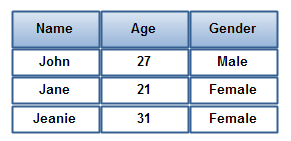
\includegraphics[scale=0.5]{imagenes/resultset.png}
\end{figure}
Para este caso el objeto \emph{ResultSet} tiene tres columnas (Name, Age, Gender) con tres registros con diferentes valores.\\
Lo podemos crear así:
\begin{lstlisting}
Statement statement = connection.createStatement();
ResultSet result = statement.executeQuery("select * from people");
\end{lstlisting}

O de esta otra manera, usando un ojbeto \emph{PreparedStatement};
\begin{lstlisting}
String sql = "select * from people";
PreparedStatement statement = connection.prepareStatement(sql);
ResultSet result = statement.executeQuery();
\end{lstlisting}
Una vez creado es típico la iteración sobre el:
\begin{lstlisting}
while(result.next()) {
    // ... get column values from this record
}
\end{lstlisting}
Accediendo al valor de las columnas:
\begin{lstlisting}
while(result.next()) {
    result.getString    (1);
    result.getInt       (2);
    result.getBigDecimal(3);
    // etc.
}
\end{lstlisting}
Actualizando con \emph{ResultSet};
\begin{lstlisting}
result.updateString     ("name", "Alex");
result.updateInt        ("age", 55);
result.updateBigDecimal ("coefficient", new BigDecimal("0.1323");
result.updateRow();
//o usando el número de columna:
result.updateString     (1, "Alex");
result.updateInt        (2, 55);
result.updateBigDecimal (3, new BigDecimal("0.1323");
result.updateRow();
\end{lstlisting}

\subsection{PreparedStatement}
Es un tipo especial de objeto \emph{Statement}, pero presenta una serie de ventajas:
\begin{enumerate}
\item Facilita la insercción de datos.
\item Reusabilidad de código.
\item Aumenta el rendimiento.
\item Permite crear procesos por lotes.
\item Evita la inyección SQL
\end{enumerate}

Ejemplo:
\begin{lstlisting}
String sql = "update people set firstname=? , lastname=? where id=?";

PreparedStatement preparedStatement =
        connection.prepareStatement(sql);

preparedStatement.setString(1, "Gary");
preparedStatement.setString(2, "Larson");
preparedStatement.setLong  (3, 123);

int rowsAffected = preparedStatement.executeUpdate();
\end{lstlisting}
En el caso de una actualización:
\begin{lstlisting}
String sql = "update people set firstname=? , lastname=? where id=?";

PreparedStatement preparedStatement =
        connection.prepareStatement(sql);

preparedStatement.setString(1, "Gary");
preparedStatement.setString(2, "Larson");
preparedStatement.setLong  (3, 123);

int rowsAffected = preparedStatement.executeUpdate();
\end{lstlisting}
Reuso de la sentencia:
\begin{lstlisting}
String sql = "update people set firstname=? , lastname=? where id=?";

PreparedStatement preparedStatement =
        connection.prepareStatement(sql);

preparedStatement.setString(1, "Gary");
preparedStatement.setString(2, "Larson");
preparedStatement.setLong  (3, 123);

int rowsAffected = preparedStatement.executeUpdate();

preparedStatement.setString(1, "Stan");
preparedStatement.setString(2, "Lee");
preparedStatement.setLong  (3, 456);

int rowsAffected = preparedStatement.executeUpdate();
\end{lstlisting}



\subsection{Batch Updates}
Nos permite agrupar sentencias SQL y enviarlas una a una, despreocupandonos de la ejecución de las mismas. Se suelen emplear con objeto \emph{Statement} y \emph{PreparedStatement}
Ejemplo:
\newpage
\begin{lstlisting}
Statement statement = null;
try{
    statement = connection.createStatement();

    statement.addBatch("update people set firstname='John' where id=123");
    statement.addBatch("update people set firstname='Eric' where id=456");
    statement.addBatch("update people set firstname='May'  where id=789");

    int[] recordsAffected = statement.executeBatch();
} finally {
    if(statement != null) statement.close();
}
\end{lstlisting}
Y otra manera:
\begin{lstlisting}
String sql = "update people set firstname=? , lastname=? where id=?";

PreparedStatement preparedStatement = null;
try{
    preparedStatement =
            connection.prepareStatement(sql);

    preparedStatement.setString(1, "Gary");
    preparedStatement.setString(2, "Larson");
    preparedStatement.setLong  (3, 123);

    preparedStatement.addBatch();

    preparedStatement.setString(1, "Stan");
    preparedStatement.setString(2, "Lee");
    preparedStatement.setLong  (3, 456);

    preparedStatement.addBatch();

    int[] affectedRecords = preparedStatement.executeBatch();

}finally {
    if(preparedStatement != null) {
        preparedStatement.close();
    }
}
\end{lstlisting}

\subsection{Transacciones}
Son un conjunto de acciones que se deben realizar de forma atómica, es decir o se hacen todas o ninguna. Las transacciones se incian con:
\begin{quote}
connection.setAutoCommit(false);
\end{quote}
En el caso que fallara alguna de las acciones, debemos volver a dejar la tabla tal y como estaba, para esto hacemos:
\begin{quote}
connection.rollback();
\end{quote}
Si todo ha funcionado debemos enviar los cambios a la BD con:
\begin{quote}
connection.commit();
\end{quote}
Esto quedaría:
\begin{lstlisting}
Connection connection = ...
try{
    connection.setAutoCommit(false);

    // create and execute statements etc.

    connection.commit();
} catch(Exception e) {
    connection.rollback();
} finally {
    if(connection != null) {
        connection.close();
    }
}
\end{lstlisting}
\newpage
Un ejemplo completo:
\begin{lstlisting}
Connection connection = ...
try{
    connection.setAutoCommit(false);


    Statement statement1 = null;
    try{
        statement1 = connection.createStatement();
        statement1.executeUpdate(
            "update people set name='John' where id=123");
    } finally {
        if(statement1 != null) {
            statement1.close();
        }
    }


    Statement statement2 = null;
    try{
        statement2 = connection.createStatement();
        statement2.executeUpdate(
            "update people set name='Gary' where id=456");
    } finally {
        if(statement2 != null) {
            statement2.close();
        }
    }

    connection.commit();
} catch(Exception e) {
    connection.rollback();
} finally {
    if(connection != null) {
        connection.close();
    }
}
\end{lstlisting}

\section{Patrones}
\subsection{Patrón Singleton}
El patrn de diseño singleton (instancia única) está diseñado para restringir la creación de objetos pertenecientes a una clase o el valor de un tipo a un único objeto.\par 
\emph{Su intención consiste en garantizar que una clase sólo tenga una instancia y proporcionar un punto de acceso global a ella.}\par 
El patrón singleton provee una única instancia global gracias a que:
\begin{itemize}
\item La propia clase es responsable de crear la única instancia.
\item Permite el acceso global a dicha instancia mediante un método de clase.
\item Declara el constructor de clase como privado para que no sea instanciable directamente.
\end{itemize}
\begin{figure}[H]
\centering
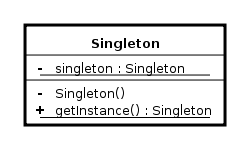
\includegraphics[scale=0.5]{imagenes/singleton.png}
\end{figure}
\newpage
Su implementación en java es la siguiente:
\begin{lstlisting}
public class SoyUnico {

    private String nombre;
    private static SoyUnico soyUnico;

    // El constructor es privado, no permite que se genere un constructor por defecto.
    private SoyUnico(String nombre) {
        this.nombre = nombre;
        System.out.println("Mi nombre es: " + this.nombre);
    }

    public static SoyUnico getSingletonInstance(String nombre) {
        if (soyUnico == null){
            soyUnico = new SoyUnico(nombre);
        }
        else{
            System.out.println("No se puede crear el objeto "+ nombre +
             " porque ya existe un objeto de la clase SoyUnico");
        }
        
        return soyUnico;
    }
    
    // metodos getter y setter

}
\end{lstlisting}

\newpage
\subsection{Patrón Singleton con jdbc}
Nos ayuda a establecer la conexión, crear una \textbf{única} conexión y manejar a nuestro antojo.
\begin{figure}[H]
\centering
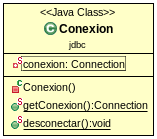
\includegraphics[scale=1]{imagenes/Conexion.png}
\end{figure}
\begin{lstlisting}
import java.sql.Connection;
import java.sql.DriverManager;
import java.sql.SQLException;
import org.sqlite.SQLiteConfig;

public class Conexion {
    private static Connection conexion = null;
    private Conexion(){}
    public static Connection getConexion(){
      if (conexion==null){
        try {
            String nombreBD = "jdbc:sqlite:ejemplo";
            SQLiteConfig config = new SQLiteConfig();  
            config.enforceForeignKeys(true);  
            Class.forName("org.sqlite.JDBC");
            conexion = DriverManager.getConnection(nombreBD, config.toProperties());
        } catch (ClassNotFoundException | SQLException e) {
            e.printStackTrace();
        }
        return conexion;
      }
    }
    public static void desconectar(){
        if (conexion != null)
           try {
              conexion.close();
           } catch (SQLException e) {
              e.printStackTrace();
           }
    }
}
\end{lstlisting}
\newpage
\subsection{Cierre de la conexión}
Java tiene mecanismos de notificación mediante los cuales podemos responder a ciertos eventos, esto mecanimos son los \emph{listener} como hemos visto en el diseño de \emph{GUI} con \emph{Swing}. Esta técnica se denominaba antiguamente como \emph{hook}.
Tenemos el evento \emph{shutdown} que corresponde a la terminación de la máquina virtual de Java pudiendo registrarlo como:
\begin{quote}
			Runtime.getRuntime().addShutdownHook(new Hook());
\end{quote}
Donde Hook es el nombre de una nueva clase que hereda de Thread y sobrescribe el método run(). La máquina virtual invocará este método antes de finalizar su ejecución, por lo que podremos cerrar aquí flujos o conexiones a BD abiertas. Ejemplo:
\begin{lstlisting}
import java.sql.Connection;
import java.sql.DriverManager;
import java.sql.SQLException;
import java.util.ResourceBundle;
public class Conexion {
   private static Connection con = null;
   public static Connection getConexion(){
        if (con == null){
            Runtime.getRuntime().addShutdownHook(new MiShutdownHuk());
            Properties p = new Properties();
            p.load(new FileReader("files/properties/config.properties"));
            String driver =  p.getString("driver");
            String url = p.getString("url");
            try {
                Class.forName(driver);
                con = DriverManager.getConnection(url);
            } catch (ClassNotFoundException e) {
                e.printStackTrace();
            } catch (SQLException e) {
                e.printStackTrace();
            }
         }
         return con;
   }
   static class MiShutdownHuk extends Thread{
      @Override
      public void run() {
         Connection con  = Conexion.getConexion();
         try {
             con.close();
         } catch (SQLException e) {
             e.printStackTrace();
         }
      }
   }
}
\end{lstlisting}
Usamos una clase interna inner class, pues su existencia esta completamente relacionada con la clase principal, la clase interna no tiene sentido por si sola.
\subsection{Patrón DAO}
\begin{itemize}
\item Patrón de diseño de software.
\item Usa una clase \emph{POJO}
\item Un solo objeto se encarga de realizar las operaciones con la BD.
\item El resto del sistema trabaja con ese objeto, aislándonos de \emph{SGBD}
\end{itemize}
\begin{figure}[H]
\centering
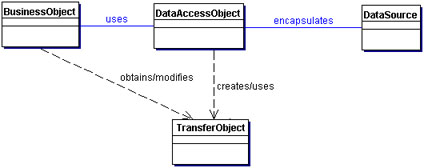
\includegraphics[scale=0.8]{imagenes/DAO.jpg}
\end{figure}
En el caso del ejercicio propuesto en la explicación del funcionamiento del SGBD \emph{sqlite} podemos aproximarnos al diagrama UML (solo una parte) con la siguiente representación:
\begin{figure}[H]
\centering
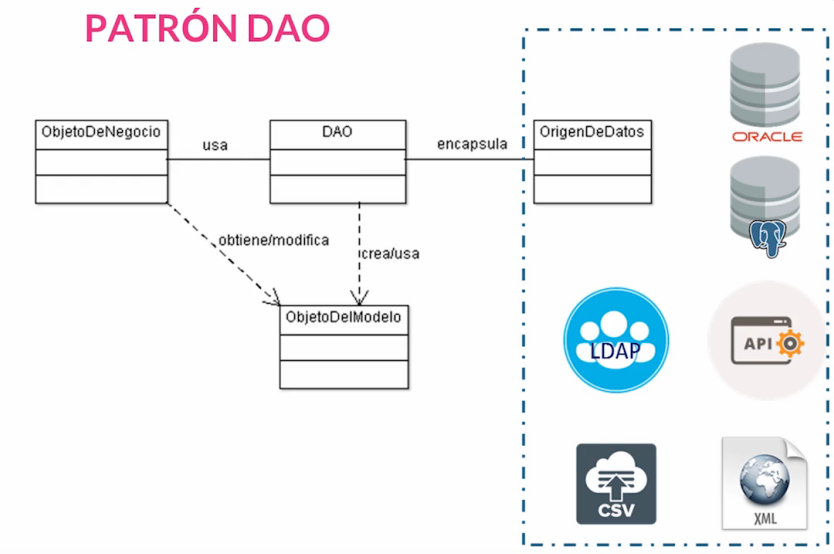
\includegraphics[scale=0.7]{imagenes/DAO.png}
\end{figure}
\newpage
Y la implementación puede quedar:\\
Para el caso de AlumnoDAO:
\begin{lstlisting}
import java.util.List;

public interface AlumnoDAO {
    void insertarAlumnoDTO(AlumnoDTO a);
    void actualizarAlumnoDTO(AlumnoDTO a, String nombre, String apellidos);
    void borrarAlumnoDTO(String nombre, String apellidos);
    List<AlumnoDTO> leerTotosAlumnos();
}
\end{lstlisting}
Y su implementación en AlumnoDTO quedará:
\begin{lstlisting}
import java.sql.Connection;
import java.sql.PreparedStatement;
import java.sql.ResultSet;
import java.sql.SQLException;
import java.sql.Statement;
import java.util.ArrayList;
import java.util.List;

public class AlumnoDAOImp implements AlumnoDAO {
    private Connection conexion = Conexion.getConexion();
	
    public void insertarAlumnoDTO(AlumnoDTO a) {
        String sql = "INSERT INTO alumno (nombre, apellidos) VALUES (?,?)";
        PreparedStatement preparedStatement=null;
        try {
            preparedStatement = conexion.prepareStatement(sql);
            preparedStatement.setString(1, a.getNombre());
            preparedStatement.setString(2, a.getApellidos());
            int rowsAffected = preparedStatement.executeUpdate();
        } catch (SQLException e1) {
            e1.printStackTrace();
        } finally {
            if (preparedStatement!=null)
               try {
                   preparedStatement.close();
               } catch (SQLException e) {
                   e.printStackTrace();
               }
        }
    }

    public void actualizarAlumnoDTO(AlumnoDTO a, String nombre, String apellidos) {
        String sqlID = "SELECT id FROM alumno WHERE nombre =? AND apellidos=?";
        String sql = "UPDATE alumno SET nombre=?, apellidos=? WHERE id= ?";
        PreparedStatement preparedstatement = null;
        ResultSet resultset =null;
        int idAlumno=0;
        try {
            preparedstatement = conexion.prepareStatement(sqlID);
            preparedstatement.setString(1,a.getNombre());
            preparedstatement.setString(2, a.getApellidos());
            resultset = preparedstatement.executeQuery();
            while(resultset.next())
                  idAlumno =resultset.getInt("id");
            preparedstatement= conexion.prepareStatement(sql);
            preparedstatement.setString(1, nombre);
            preparedstatement.setString(2, apellidos);
            preparedstatement.setInt(3, idAlumno);
            int rowsAffected = preparedstatement.executeUpdate();
        } catch (SQLException e) {
            e.printStackTrace();
        } finally {
            if (resultset != null)
               try {
                   resultset.close();
               } catch (SQLException e) {
                   e.printStackTrace();
               }
            if (preparedstatement != null)
               try {
                   preparedstatement.close();
               } catch (SQLException e) {
                   e.printStackTrace();
               }
        }
		
		
     }
	
     public void borrarAlumnoDTO(String nombre, String apellidos) {
        String sql = "DELETE FROM alumno WHERE nombre =? AND apellidos=?";
        PreparedStatement preparedstatement = null;
        ResultSet resultset =null;
        try {
            preparedstatement = conexion.prepareStatement(sql);
            preparedstatement.setString(1,nombre);
            preparedstatement.setString(2, apellidos);
            int rowsAffected = preparedstatement.executeUpdate();
        } catch (SQLException e) {
            e.printStackTrace();
        } finally {
            if (resultset != null)
               try {
                   resultset.close();
               } catch (SQLException e) {
                   e.printStackTrace();
               }
            if (preparedstatement != null)
               try {
                   preparedstatement.close();
               } catch (SQLException e) {
                   e.printStackTrace();
               }
        }
    }
	
    public List<AlumnoDTO> leerTotosAlumnos() {
        List<AlumnoDTO> lista= new ArrayList<AlumnoDTO>();
        String sql = "SELECT * FROM alumno";
        Statement statement = null;
        ResultSet resultset = null;
        AlumnoDTO a;
        String nombre, apellidos;
        try {
            statement = conexion.createStatement();
            resultset = statement.executeQuery(sql);
            while (resultset.next()) {
                  nombre = resultset.getString("nombre");
                  apellidos = resultset.getString("apellidos");
                  a = new AlumnoDTO(nombre, apellidos);
                  lista.add(a);
            }
        } catch (SQLException e) {
            e.printStackTrace();
        } finally {
            if (resultset != null)
               try {
                   resultset.close();
               } catch (SQLException e) {
                   e.printStackTrace();
               }
            if (statement != null)
               try {
                   statement.close();
               } catch (SQLException e) {
                    e.printStackTrace();
               }
        }
        return lista;
    }
}
\end{lstlisting}

\section{Bibliografía}
La parte inicial está obtenida de este tutorial:\par 
\textbf{\emph{\href{http://tutorials.jenkov.com/jdbc/index.html}{Tutorial JDBC de Jakob Jenkov}}}\par 
\textbf{\emph{\href{http://www.javamexico.org/blogs/richardmx/que_es_data_access_object}{Explicación DAO de javamexico}}}\par
\textbf{\emph{\href{http://www.tutorialspoint.com/jdbc/}{Tutorial jdbc de tutorialspoint}}}\par
\textbf{\emph{\href{http://jarroba.com/patron-singleton-en-java-con-ejemplos/}{Tutorial patrón Singleton en jarroba}}}

\end{document}

